\section{Pregunta 10}

\subsection{Enunciado del Problema:}
Los autores del articulo sobre lottery scheduling alegan que la optimizacion de compensation tickets es necesaria para compensar una posible falencia del algoritmo inicialmente propuesto en ciertos escenarios. Disenar y llevar a cabo un experimento apropiado para comprobar esta afirmacion (provocar un escenario donde se manifieste el problema, comparar simulaciones ejecutadas con y sin compensation tickets y discutir los resultados obtenidos).

\subsection{Solución}
Dado que lo que queremos ver es que la optimizacion de \textit{Compensation tickets} es necesaria, mostraremos que en un escenario propuesto por nosotros el \textit{lottery scheduling} es menos justo con la asignación del CPU a los procesos si no utiliza el \textit{compensation ticket}.

El escenario propuesto es el siguiente:
\begin{itemize}
	\item Fijaremos el quantum en 4 ciclos de clock.
	\item Fijaremos el costo de cambio de contexto y el costo de cambio de núcleo en cero ciclos de clock para que no entorpezcan las mediciones.
	\item Fijaremos el numero de núcleos de procesamiento en uno.
\end{itemize}


Ademas, utilizaremos el siguiente lote de tareas:
\begin{quote}
TaskCPU 35\\
TaskCPU 35\\
TaskBatch 9 9\\
\end{quote}


Elegimos este lote para tener dos procesos que utilizan intensivamente el CPU compitiendo continuamente por el CPU y que, al deshabilitar el \textit{Compensation Ticket}, obliguen al proceso TaskBatch a esperar mucho antes de poder utilizar el CPU.

Ademas, cada vez que el proceso TaskBatch gane el CPU, lo utilizara por un solo ciclo y luego se bloqueara (por como esta implementado TaskBatch).
Se hace eligio esto para minimizar la cantidad de quantum que la tareas bloqueante utiliza y así maximizar la cantidad de tickets que obtendrá el proceso por los Compensation Tickets.\\

Es importante señalar que probamos con muchos otros lotes de tareas y, en todos ellos, obteníamos el resultado inverso al esperado, es decir, la experimentación daba como resultado que el algoritmo sin compensation ticket era mas justo que con.
Con este lote de tareas no sucede eso, y ese fue otro de los motivos por el cual lo elegimos.

Utilizaremos la métrica descrita en el \textbf{Ejercicio 9} para medir el \textit{fairness} del algoritmo, y llevaremos a cabo la medición hasta el tick 42 del procesador, por los motivos que explicamos en el ejercicio anterior.\\


A continuación, exponemos los resultados de la experimentación utilizando el Compensation Ticket y el lote descrito:


\begin{figure}[H]
\begin{center}
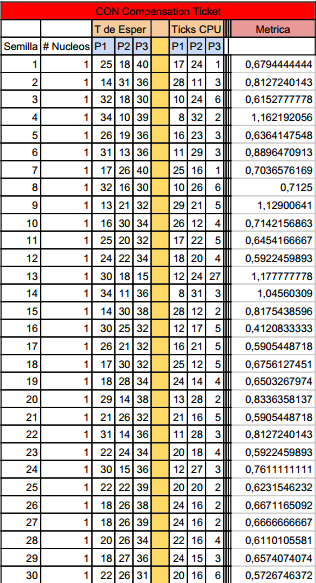
\includegraphics[width=0.6\textwidth]{img/refotaza1.png}
     \caption{Lottery Scheduling con Compensation Tickets hasta el tick 42}
\end{center}
\end{figure}

Ahora, si llevamos a cabo la misma experimentación, pero \textbf{sin Compensation Ticket} resulta en el siguiente gráfico:

\begin{figure}[H]
\begin{center}
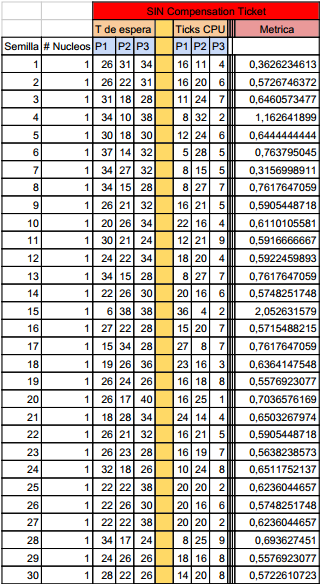
\includegraphics[width=0.6\textwidth]{img/refotaza2.png}
     \caption{Scheduling lottery sin Compensation Tickets hasta el tick 42}
\end{center}
\end{figure}


Ahora, para comparar los resultados obtenidos en ambos experimentos, calcularemos la esperanza, la varianza y el desvió estándar de ambas muestras.
El resultado es el siguiente:
\begin{figure}[H]
\begin{center}
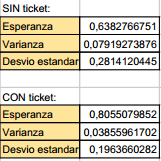
\includegraphics[width=0.3\textwidth]{img/refotaza3.png}
     \caption{Esperanza, Varianza, y Desvió estándar de las muestras}
\end{center}
\end{figure}

Como se puede observar, tanto la varianza como el desvió estándar son mayores cuando el algoritmo no utiliza el Compensation Ticket, es decir, el intervalo en el cual se haya la esperanza $(\mu - \sigma, \mu + \sigma)$ es mayor y, por lo tanto, podemos concluir que el algoritmo es menos justo asignando el CPU.
Luego, podemos concluir que en ciertos escenarios, la optimizacion del Compensation Ticket es necesaria, pues sin el Compensation ticket la asignación del CPU es menos justa.
